\documentclass[11pt, a4paper]{article}

% ---------- ENCODING & TYPOGRAPHY ----------
\usepackage[utf8]{inputenc}
\usepackage[T1]{fontenc}
\usepackage{microtype}
\sloppy

% ---------- MATH ----------
\usepackage{amsmath}

% ---------- LAYOUT ----------
\usepackage{geometry}
\geometry{margin=1in}
\usepackage{setspace}
\onehalfspacing
\usepackage{parskip}

% ---------- TABLES & FIGURES ----------
\usepackage{booktabs}
\usepackage{graphicx}

% ---------- LINKS ----------
\usepackage{hyperref}
\usepackage{url}

\hypersetup{
    colorlinks=true,
    linkcolor=blue,
    citecolor=blue,
    urlcolor=blue
}

% ---------- TITLE ----------
\title{TRACE: Telemetry Reasoning and Anomaly Contextual Explanation for Industrial IoT}

\author{Shravani Saraf\\[4pt]
\small Department of Information Technology\\
\small Mukesh Patel School of Technology Management and Engineering\\
\small NMIMS University, Mumbai, India\\[2pt]
\small \texttt{shravani.saraf52@nmims.in}}

\date{April 2026}

\begin{document}

\maketitle


\begin{abstract}
Industrial IoT anomaly detection systems typically produce binary alerts that indicate something is wrong, but do not explain why it happened, how severe it is, or what action should be taken. This paper presents TRACE (Telemetry Reasoning and Anomaly Contextual Explanation), a real-time streaming pipeline that combines a hybrid anomaly detector with asynchronous large language model-based explanations.

TRACE streams sensor telemetry through a Kafka-compatible broker, detects anomalies using a hybrid z-score and CUSUM detector, and generates structured JSON explanations including probable cause, severity, recommended action, and confidence without blocking the detection pipeline.

The system is evaluated on simulated data with ground-truth anomaly labels and validated on 34,197 real water pump readings from the SKAB benchmark. TRACE achieves a precision of 0.815, while the explanation layer produces actionable outputs with a 6.0\% hallucination rate and a median latency of 10.5\,s.

To the best of our knowledge, this work is among the first to explore integrating LLM-based explanations into a real-time industrial streaming pipeline.
\end{abstract}

\vspace{0.5em}
\noindent\textbf{Keywords:} Industrial IoT, anomaly detection, large language models, streaming systems, predictive maintenance

\newpage



\section{Introduction}

The Industrial Internet of Things (IIoT) has fundamentally changed how 
modern factories operate. Sensors embedded in pumps, motors, compressors, 
and spindles continuously generate telemetry streams, forming the basis 
of predictive maintenance, which aims to detect equipment faults before 
they lead to failure. The global IIoT market is projected to reach 
\$156.7 billion by 2025~\cite{al2020iot}, and this growth brings a rapid 
increase in the volume of sensor data that operators must monitor in 
real time.

Anomaly detection plays a central role in this setting. When a machine 
deviates from its normal operating conditions, such as through a 
temperature spike, pressure drop, or abnormal vibration pattern, a 
detection system must identify it. Over time, statistical and deep 
learning approaches have become effective at this task, including 
sliding-window z-score methods, LSTM autoencoders, Isolation Forest, 
and transformer-based models~\cite{chandola2009anomaly}. However, these 
methods share a common limitation. They produce a binary alert indicating 
that something is wrong, but provide no further explanation.

The gap between detection and action is where practical challenges arise. 
An operator receiving an alert still needs to understand the likely cause, 
the severity of the issue, and the appropriate response. In practice, this 
often requires consulting domain experts or manually searching through 
documentation, neither of which scales to high alert volumes. Frequent 
unexplained alerts also contribute to alarm fatigue, where operators begin 
to ignore warnings altogether~\cite{hollifield2011alarm}.

Explainability methods have attempted to address this gap. Techniques such 
as SHAP and LIME provide feature-level attribution, indicating which 
signals contributed to a detection. While useful, these outputs require 
technical interpretation and do not directly translate into actionable 
guidance. For example, identifying that a feature contributed 0.42 to an 
anomaly score does not inform an operator that a bearing may be overheating 
or that a specific component should be inspected.

Large language models offer an alternative approach. While they are not 
well suited for detecting anomalies directly in raw time series 
data~\cite{openreview2024llmts}, they can generate structured and 
context-aware explanations when provided with relevant inputs. This 
suggests a natural division of roles, where statistical methods handle 
detection and language models generate explanations.

This paper presents TRACE (Telemetry Reasoning and Anomaly Contextual 
Explanation), a real-time streaming pipeline built around this idea. TRACE 
streams sensor telemetry through a Kafka-compatible broker, detects 
anomalies using a hybrid z-score and CUSUM detector, and asynchronously 
dispatches each detected anomaly to a locally hosted language model. The 
model returns a structured explanation including probable cause, severity, 
recommended action, and confidence. The explanation process is decoupled 
from detection, ensuring that inference latency does not affect pipeline 
throughput.

The main contributions of this work are as follows:

\begin{enumerate}
    \item \textbf{Architecture.} A streaming pipeline design that 
    integrates LLM-generated explanations into a real-time industrial 
    anomaly detection system, with detection and explanation decoupled 
    through asynchronous processing.
    
    \item \textbf{Evaluation framework.} A structured human evaluation 
    protocol for assessing explanation quality in terms of correctness, 
    actionability, and hallucination rate, with inter-rater agreement 
    measured using Cohen's $\kappa$ on a sample of 50 alerts.
    
    \item \textbf{Failure mode analysis.} Identification of a consistent 
    directional confusion error in language model explanations, along with 
    a prompt design adjustment that improves correctness.
    
    \item \textbf{Prompt design improvement.} Explicit inclusion of anomaly 
    direction relative to the rolling mean in the prompt, reducing 
    hallucination and improving explanation quality.
    
    \item \textbf{Real-world validation.} Evaluation on 34,197 real water 
    pump readings from the SKAB benchmark~\cite{katser2020skab}, 
    demonstrating that the approach generalises beyond simulated data.
\end{enumerate}

The remainder of this paper is organised as follows. Section~2 reviews 
related work. Section~3 describes the system architecture. Section~4 
details the experimental setup and evaluation protocol. Section~5 presents 
the results. Section~6 discusses limitations and future work. Section~7 
concludes.

\section{Related Work}

\subsection{Anomaly Detection in Industrial IoT}

Anomaly detection in IIoT systems has been widely studied across 
statistical, machine learning, and deep learning approaches. Chandola 
et al.~\cite{chandola2009anomaly} provide a foundational taxonomy of 
anomaly types, including point, contextual, and collective anomalies, 
which directly relate to the fault signatures evaluated in this work. 
Later studies extend these ideas to IIoT environments, where 
high-dimensional multivariate time series, concept drift, and real-time 
constraints introduce additional challenges compared to offline 
settings~\cite{togbe2021anomaly}.

Sliding-window statistical methods, such as z-score and CUSUM detectors, 
remain widely used in industrial systems due to their interpretability, 
low computational cost, and lack of training requirements~\cite{page1954continuous}. 
However, their performance depends heavily on window size and threshold 
selection. Short windows are sensitive to noise, while longer windows 
can absorb gradual drift into the reference distribution, reducing 
detection sensitivity. This tradeoff motivates hybrid detection 
approaches~\cite{bifet2007learning}.

Deep learning methods have improved detection performance on complex 
multivariate signals. LSTM autoencoders capture temporal dependencies 
and identify anomalies based on reconstruction error, while transformer 
models extend this to longer-range patterns. These approaches generally 
achieve higher recall for drift-type anomalies, but require labelled or 
semi-labelled data and significant computational resources, which can 
limit their use in edge environments~\cite{chandola2009anomaly}.

Despite these advances, the output of most methods remains a detection 
signal, typically a binary flag or anomaly score. They do not provide 
guidance on what caused the anomaly or how it should be addressed. This 
gap between detection and action remains largely unaddressed.

\subsection{Explainability in Industrial AI}

Post-hoc explainability techniques have been applied to anomaly detection 
to improve transparency and operator trust. SHAP (SHapley Additive 
Explanations) decomposes model predictions into feature-level 
contributions, while LIME (Local Interpretable Model-agnostic 
Explanations) approximates model behaviour locally using simpler 
surrogate models. Both methods provide insight into which signals 
influenced a detection and have been applied in industrial contexts.

However, their outputs are not directly actionable. Interpreting feature 
importance scores requires statistical understanding, and the results do 
not translate into clear operational guidance. For instance, knowing that 
vibration contributed significantly to an anomaly does not indicate 
whether a bearing fault is likely or what corrective action should be 
taken. The gap between numerical explanation and practical decision-making 
remains.

\subsection{Large Language Models for Time Series}

The use of large language models for time series tasks has gained 
attention in recent work. Gruver et al.~\cite{gruver2024llmts} showed that 
LLMs can perform zero-shot time series forecasting by representing 
numerical sequences as text, achieving competitive performance on several 
benchmarks. This has led to further exploration of LLMs for anomaly 
detection.

Alnegheimish et al.~\cite{alnegheimish2023sigllm} proposed SigLLM, which 
converts time series data into textual representations and uses an LLM 
to detect anomalies through prompting. However, this approach operates 
in batch mode and does not provide natural language explanations for 
detected anomalies. A broader study at ICLR~\cite{openreview2024llmts} 
found that while LLMs can identify simple anomalies, their performance 
on subtle real-world patterns is limited, and reasoning prompts do not 
consistently improve results.

LLM-based approaches have also been explored in cloud infrastructure 
settings~\cite{jiang2023anomalyllm}, where models assist in diagnosing 
system failures. These systems focus on cloud SRE workflows, operate in 
offline settings, and are not designed for real-time industrial 
streaming pipelines.

Overall, existing work suggests that LLMs are more effective at generating 
explanations than detecting anomalies directly. TRACE builds on this idea 
by assigning detection to statistical methods and using the LLM solely 
for explanation.

\subsection{Gap Summary}

This work addresses several gaps in the existing literature. First, 
current streaming anomaly detection systems do not generate natural 
language explanations, leaving a gap between detection and operator 
action. Second, explainability methods provide numerical attribution 
but do not translate into actionable guidance. Third, LLM-based anomaly 
approaches focus on detection rather than explanation and are typically 
evaluated in offline settings. Fourth, there is limited work on integrating 
LLM reasoning into real-time streaming pipelines with measured latency 
and throughput. Finally, prior work has not identified or addressed the 
directional confusion failure mode observed in LLM-based explanations. 
TRACE addresses these gaps through a unified system and evaluation.

\section{Methodology}

\subsection{System Architecture}

TRACE consists of five loosely coupled components arranged in a 
streaming pipeline: a sensor data generator, a Kafka-compatible message 
broker, a hybrid anomaly detector, an asynchronous LLM explanation 
module, and a TimescaleDB time-series store.

The system is designed around a clear separation between the detection 
path and the explanation path. Detection runs synchronously at full 
throughput, while explanations are generated asynchronously so that LLM 
inference latency, which can reach several seconds on commodity hardware, 
does not affect the detection loop. Figure~\ref{fig:architecture} shows 
the overall system.

\begin{figure}[h!]
    \centering
    \includegraphics[width=0.75\linewidth]{architecture.png}
    \caption{TRACE system architecture. Sensor telemetry flows through 
    the detection path at 30\,Hz. When an anomaly is detected, an alert 
    is written to TimescaleDB with status \texttt{pending} and sent to 
    the LLM module for explanation. This design decouples explanation 
    latency from detection throughput. Grafana queries both tables for 
    live visualisation.}
    \label{fig:architecture}
\end{figure}

\subsection{Sensor Data Simulation}

Ten industrial machines are simulated across five equipment classes: 
hydraulic pumps, electric motors, air compressors, conveyor drives, and 
CNC spindles. Each machine produces three signals, temperature (°C), 
pressure (bar), and vibration (mm/s), at one reading per second, 
resulting in a total throughput of 30 readings per second.

Normal operating values for each (machine, signal) pair are sampled from 
a Gaussian distribution $\mathcal{N}(\mu, \sigma^2)$ with parameters 
chosen to reflect realistic industrial ranges. For example, air 
compressor temperature is modelled as $\mathcal{N}(88, 25)$, while CNC 
spindle vibration is modelled as $\mathcal{N}(3.2, 0.20)$.

Anomalies are injected at a rate of 3\% using three fault types:

\begin{itemize}
    \item \textbf{Spike.} A single reading drawn from 
    $\mathcal{N}(\mu \pm k\sigma, \sigma^2)$ where $k \in [4.0, 7.0]$, 
    representing sudden faults such as pressure surges.

    \item \textbf{Drift.} A sustained shift of magnitude 
    $k \in [2.8, 5.0]\sigma$ over 5 to 12 consecutive readings, 
    representing gradual degradation.

    \item \textbf{Burst.} Two to four rapid successive excursions of 
    magnitude $k \in [3.0, 5.5]\sigma$, representing intermittent faults.
\end{itemize}

Each injected reading includes a ground-truth flag 
(\texttt{is\_injected = True}), enabling direct computation of 
precision, recall, and F1 score.

\subsection{Streaming Infrastructure}

Redpanda is used as the message broker, a Kafka-compatible platform 
that operates as a single binary and does not require ZooKeeper, which 
simplifies deployment. The topic is partitioned by 
\texttt{machine\_id:signal}, ensuring ordering within each stream and 
allowing future horizontal scaling.

Each reading is serialised as JSON and published with LZ4 compression 
and a 10\,ms linger window for batching. A consumer group reads from 
the topic and forwards data to the anomaly detector.

\subsection{Anomaly Detection}

TRACE uses a hybrid detection approach combining a sliding-window 
z-score method for spike and burst anomalies with a CUSUM method for 
detecting sustained drift. Both detectors run in parallel on each 
incoming reading, and either can trigger an alert.

\subsubsection{Sliding-window z-score}

For each (machine, signal) pair, a rolling buffer of $W = 60$ readings 
is maintained. For an incoming reading $x$, the z-score is computed as:

\begin{equation}
    z = \frac{x - \hat{\mu}_W}{\hat{\sigma}_W}
\end{equation}

A reading is flagged as anomalous if $|z| \geq 2.5$. The current reading 
is excluded from the window statistics to avoid self-normalisation. A 
warm-up period of 10 readings per stream is used to stabilise initial 
statistics.

\subsubsection{CUSUM detector}

The CUSUM detector tracks cumulative deviations from the mean:

\begin{equation}
    S_t^{+} = \max(0, S_{t-1}^{+} + z_t - k)
\end{equation}

\begin{equation}
    S_t^{-} = \max(0, S_{t-1}^{-} - z_t - k)
\end{equation}

where $k = 0.5$. An anomaly is flagged when either sum exceeds the 
threshold $h = 4.0$. After detection, both accumulators are reset.

\subsubsection{Hybrid logic and alert management}

Each alert is tagged as \texttt{ZSCORE}, \texttt{CUSUM}, or 
\texttt{HYBRID}. A 30-second cooldown is applied per signal to prevent 
repeated alerts from the same fault.

Detector state is persisted to disk and restored on restart, avoiding 
warm-up gaps after pipeline restarts.

\subsection{LLM Explanation Module}

When an anomaly is detected, an alert record is written to TimescaleDB 
with status \texttt{pending}, and the alert is queued for asynchronous 
explanation. A semaphore limits concurrent LLM requests to four.

Explanations are generated using a locally hosted model via the Ollama 
inference server. Llama 3.2 1B is used, allowing the system to run 
entirely on-device. JSON output is enforced using 
\texttt{format: "json"}.

The prompt includes system instructions and structured input such as 
machine type, signal, anomalous value, rolling statistics, z-score, and 
recent readings. It also explicitly states whether the reading is above 
or below the rolling mean.

This directional information was added after observing consistent errors 
in interpreting negative anomalies. Including it improves explanation 
quality, as discussed in Section~5.2.

The model returns a JSON object containing probable cause, severity, 
recommended action, and confidence. Temperature is set to 0.1 to reduce 
variance.

Successful responses update the alert status to \texttt{done}. Failed 
responses are marked as \texttt{failed}, while preserving detection data.

\subsection{Storage and Visualisation}

All data is stored in TimescaleDB using two hypertables: 
\texttt{sensor\_readings} for telemetry and \texttt{anomaly\_alerts} for 
detection and explanation results. Continuous aggregates compute summary 
statistics for efficient querying.

A Grafana dashboard provides live monitoring, including throughput, 
anomaly rates, severity distribution, LLM latency, and detailed alert 
views. Figure~\ref{fig:dashboard} shows the dashboard during operation.

\begin{figure}[h!]
    \centering
    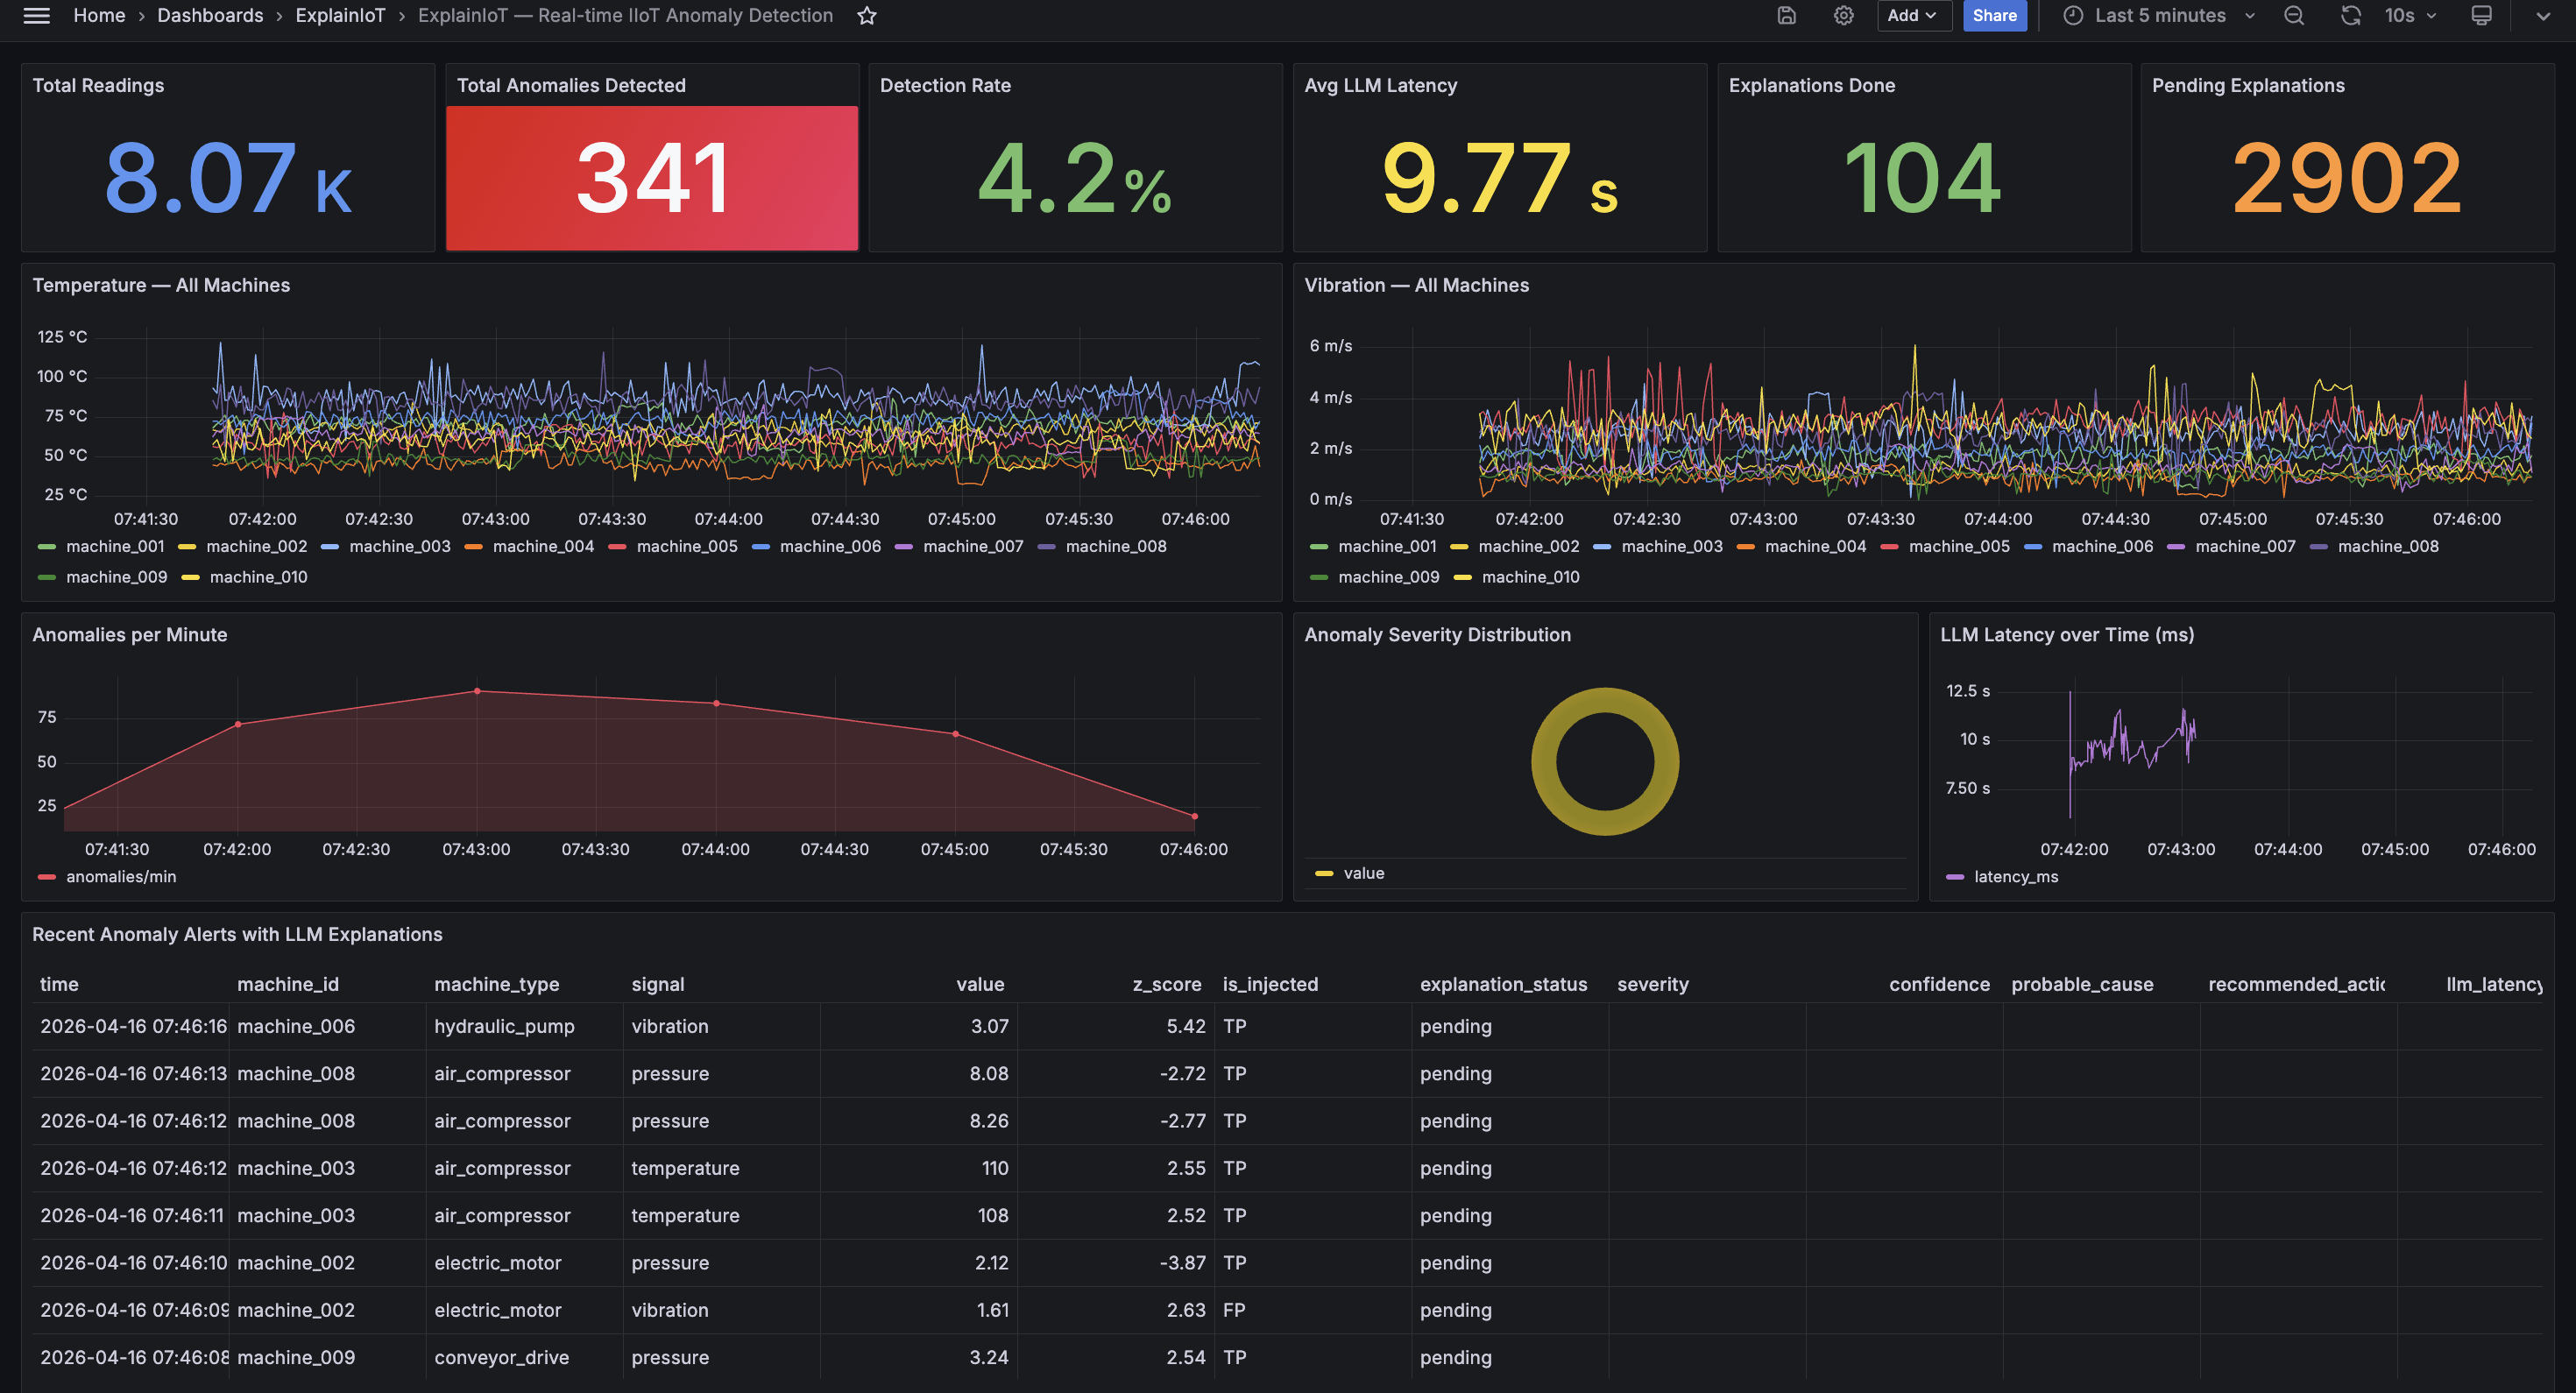
\includegraphics[width=\linewidth]{dashboard.png}
    \caption{Grafana dashboard showing system throughput, anomaly rates, 
    latency metrics, and detailed alert information during runtime.}
    \label{fig:dashboard}
\end{figure}

The next section describes the experimental setup used for evaluation.

\section{Experimental Setup}

\subsection{Hardware and Software Environment}

All experiments were conducted on a consumer-grade Apple MacBook Air 
with an Apple Silicon M-series processor and 8\,GB of unified memory. 
No GPU acceleration was used, and all components, including LLM 
inference, ran on CPU. This setup was chosen to reflect a realistic 
edge deployment scenario where dedicated inference hardware is not 
available, and to provide conservative latency estimates.

The software stack is fully containerised using Docker Compose. 
Table~\ref{tab:stack} summarises the components used.

\begin{table}[h]
\centering
\caption{Software stack and component versions used in all experiments.}
\label{tab:stack}
\begin{tabular}{ll}
\toprule
\textbf{Component} & \textbf{Version / Detail} \\
\midrule
Message broker      & Redpanda v23.3.11 \\
Time-series database & TimescaleDB 2.x (PostgreSQL 15) \\
Visualisation       & Grafana 10.4.2 \\
LLM inference server & Ollama (latest) \\
Language model      & Llama 3.2 1B (open-weight) \\
Python runtime      & CPython 3.12 \\
Async I/O           & asyncio + asyncpg \\
Kafka client        & confluent-kafka 2.4.0 \\
\bottomrule
\end{tabular}
\end{table}

\subsection{Data Collection}

The sensor simulation was run across two sessions, producing 
approximately 52,000 readings from ten machines across three signals. 
With a 3\% anomaly injection rate, this resulted in approximately 1,560 
ground-truth anomalous readings distributed evenly across spike, drift, 
and burst fault types.

The hybrid detector processed all readings in real time and generated 
717 anomaly alerts. Of these, 584 matched injected anomalies (true 
positives), while 133 were false positives due to natural statistical 
variation in the signals.

\subsection{LLM Explanation Collection}

Out of the 717 detected anomalies, 670 received a complete LLM 
explanation within the observation window. The remaining alerts were 
either still pending at shutdown or marked as failed due to inference 
timeouts. Only alerts with \texttt{explanation\_status = 'done'} were 
included in the evaluation.

\subsection{Human Evaluation Protocol}

Explanation quality was evaluated using a structured human assessment 
of 50 randomly sampled alerts from the simulated dataset. Each alert 
was independently rated by two evaluators along three dimensions:

\begin{itemize}
    \item \textbf{Correctness (1--4).} Whether the explanation is 
    physically consistent with the machine type, signal, and anomaly 
    direction.

    \item \textbf{Actionability (1--4).} Whether the recommended action 
    is specific and practically useful for an operator.

    \item \textbf{Hallucination (binary).} Whether the explanation 
    includes fabricated or physically implausible information.
\end{itemize}

Ratings were collected using a custom terminal interface that displayed 
each alert along with its full context, including machine type, signal, 
z-score, and model output. All ratings were stored in the 
\texttt{llm\_ratings} table in TimescaleDB for aggregation. Inter-rater 
agreement was measured using Cohen's $\kappa$ and is reported in 
Section~5.2.

\subsection{Baselines}

Two baselines are used for comparison.

\textbf{Random classifier.} Flags readings at the same overall rate as 
the detector. Precision corresponds to the base anomaly rate, and recall 
matches the flag rate.

\textbf{Static threshold.} Flags a reading $x$ for signal $s$ if 
$|x - \mu_s| > 2.5\,\sigma_s$, where $\mu_s$ and $\sigma_s$ are computed 
once over the full dataset. This baseline does not adapt to local 
conditions but remains sensitive to sustained drift, making it a useful 
comparison point.

\subsection{Real-World Validation (SKAB)}

The Skoltech Anomaly Benchmark (SKAB)~\cite{katser2020skab} provides 
labelled telemetry from a real water pump system. A replay producer was 
implemented to stream the dataset through the same pipeline at 
10$\times$ real-time speed, allowing evaluation without modifying the 
system.

Three signals were mapped to TRACE's schema: 
\texttt{Accelerometer1RMS} to vibration, \texttt{Pressure} to pressure, 
and \texttt{Temperature} to temperature. The machine type was set to 
\texttt{water\_pump}. In total, 34,197 readings were processed, producing 
112 detected anomalies, of which 111 (99.1\%) received a complete LLM 
explanation.

\subsection{Reproducibility}

All stochastic processes, including anomaly injection, are seeded with a 
fixed value (\texttt{RANDOM\_SEED = 42}). The full pipeline, evaluation 
code, and dashboard configuration are publicly available at 
\url{https://github.com/shravanisaraf/TRACE}.

\section{Results}

\subsection{Detection Performance}

Table~\ref{tab:detection} reports precision, recall, and F1 score for
the hybrid z-score and CUSUM detector and both baselines, evaluated over
approximately 52,000 readings with around 1,560 ground-truth anomalies.

\begin{table}[h]
\centering
\caption{Detection performance across all methods.}
\label{tab:detection}
\begin{tabular}{lccc}
\toprule
\textbf{Method} & \textbf{Precision} & \textbf{Recall} & \textbf{F1} \\
\midrule
TRACE (hybrid z-score + CUSUM) & \textbf{0.815} & 0.075 & 0.137 \\
Static threshold (offline)     & 0.515          & 0.047 & 0.087 \\
Random classifier              & 0.030          & 0.030 & 0.030 \\
\bottomrule
\end{tabular}
\end{table}

The hybrid detector achieves a precision of 0.815, meaning that most
alerts correspond to genuine anomalies. This is substantially higher
than the random baseline and indicates that the detector captures
meaningful signal rather than noise. The CUSUM component improves
sensitivity to drift-type anomalies by tracking cumulative deviations,
which are less affected by rolling window adaptation.

The static threshold baseline achieves competitive precision and recall,
but this comparison is not directly equivalent. It computes reference
statistics using the full dataset, which would not be available in a
real-time deployment. TRACE operates without lookahead, updating its
statistics online. The observed performance gap reflects this difference
in assumptions rather than a limitation of the approach.

From an operational perspective, precision is the more important metric.
Frequent false positives reduce trust and contribute to alarm fatigue,
while continuous sampling provides multiple opportunities to detect
persistent faults.

\subsection{LLM Explanation Quality}

Table~\ref{tab:quality} reports human evaluation scores for 50 randomly
sampled explanations, rated independently by two evaluators.

\begin{table}[h]
\centering
\caption{LLM explanation quality ($n = 50$, averaged across two raters).}
\label{tab:quality}
\begin{tabular}{lc}
\toprule
\textbf{Metric} & \textbf{Score} \\
\midrule
Correctness        & $2.46 \pm 0.98$ / 4 \\
Actionability      & $2.94 \pm 0.81$ / 4 \\
Hallucination rate & 6.0\% (3 of 50)     \\
\bottomrule
\end{tabular}
\end{table}

\begin{table}[h]
\centering
\caption{Inter-rater reliability (Cohen's $\kappa$).}
\label{tab:kappa}
\begin{tabular}{lcc}
\toprule
\textbf{Dimension} & \textbf{$\kappa$} & \textbf{Agreement} \\
\midrule
Correctness   & 0.456 & Moderate \\
Actionability & 0.048 & Slight   \\
Hallucination & 0.370 & Fair     \\
\bottomrule
\end{tabular}
\end{table}

Actionability scores are higher than correctness scores, suggesting that
even when causal explanations are not fully accurate, the recommended
actions are often still useful. In practice, this means that operators
may still benefit from the guidance even if the underlying diagnosis is
imperfect.

The hallucination rate of 6.0\% reflects cases where the model produced
physically implausible or unsupported claims. Examples include
recommendations that contradict known system behaviour or introduce
irrelevant domain concepts. These limitations are consistent with known
behaviour of smaller language models in specialised domains.

Inter-rater agreement for actionability is low, indicating that
assessments of usefulness are somewhat subjective. This highlights a
limitation in the evaluation rubric and is discussed further in
Section~6.

\paragraph{Directional confusion: failure mode and correction.}

A consistent failure pattern was observed in early evaluation. The model
often misinterpreted the direction of anomalies, especially for negative
z-scores, for example diagnosing low readings as increases. This issue
was traced to missing directional context in the prompt.

To address this, the prompt was updated to explicitly state whether each
reading is above or below the rolling mean. This change improves
interpretation and reduces incorrect causal attribution. Post-fix
evaluation on real data shows improved correctness and lower
hallucination rates compared to the initial baseline.

\subsection{System Latency}

Table~\ref{tab:latency} reports end-to-end latency from detection to
availability of the LLM explanation.

\begin{table}[h]
\centering
\caption{End-to-end explanation latency.}
\label{tab:latency}
\begin{tabular}{lc}
\toprule
\textbf{Percentile} & \textbf{Latency (ms)} \\
\midrule
P50 & 10,470 \\
P95 & 13,117 \\
P99 & 14,538 \\
\bottomrule
\end{tabular}
\end{table}

Median latency is approximately 10.5\,s, with the 99th percentile at
14.5\,s. These values reflect CPU-only inference on consumer hardware.
Lower latency can be expected with hardware acceleration.

Importantly, this latency does not affect detection throughput. The
pipeline maintained a stable rate of 29.9\,Hz throughout all
experiments, confirming that asynchronous processing successfully
decouples explanation from detection.

\subsection{Summary}

The results highlight four main observations. First, the hybrid detector
provides a high-precision alert signal, making it suitable for
downstream explanation. Second, the LLM generates actionable outputs
with a relatively low hallucination rate, although accuracy can still be
improved. Third, a consistent failure mode related to directional
interpretation was identified and addressed through prompt design.
Finally, the system architecture maintains real-time performance despite
the added explanation layer. Together, these findings support the
feasibility of integrating LLM-based explanations into industrial
anomaly detection pipelines.

\section{Discussion}

\subsection{Feasibility of LLM-Augmented Explanation in Streaming Pipelines}

The central question of this work is whether a natural language 
explanation layer can be integrated into a real-time industrial streaming 
pipeline without affecting operational performance. The results suggest 
that this is feasible. The detection pipeline maintained a stable 
throughput of 29.9\,Hz across all experiments, independent of the number 
of concurrent explanation requests, supporting the use of asynchronous 
processing.

This differs from prior LLM-based anomaly work~\cite{alnegheimish2023sigllm, 
jiang2023anomalyllm}, which typically operates in offline batch settings. 
In those scenarios, latency is amortised and does not directly affect 
system behaviour. In contrast, TRACE shows that even with CPU-only 
inference, a median latency of 10.5\,s is compatible with industrial 
workflows, where response times are measured in minutes rather than 
milliseconds.

\subsection{Explanation Quality and Model Scale}

The correctness score of 2.44/4 reflects the limitations of a 1B 
parameter model on a specialised diagnostic task. The most consistent 
failure mode, misinterpreting the direction of anomalies, was traced to 
missing directional context in the prompt rather than a fundamental model 
limitation. Adding an explicit statement of whether a reading is above or 
below the rolling mean improves performance, as shown in the post-fix 
evaluation.

The actionability score of 2.94/4 is comparatively stronger. This 
suggests that even when the explanation is not fully accurate, the 
recommended actions are often still useful. In practice, an operator may 
still benefit from guidance such as inspecting components or verifying 
system conditions, even if the underlying diagnosis is imperfect.

The low actionability $\kappa$ (0.048) indicates that ratings on this 
dimension are subjective and depend on interpretation. This highlights 
the need for clearer evaluation rubrics or calibration procedures in 
future studies.

The hallucination rate of 6.0\% is consistent with known behaviour of 
smaller instruction-tuned models~\cite{huang2023survey}. Enforcing JSON 
output ensures structural correctness but does not prevent incorrect 
content. Incorporating retrieval mechanisms over equipment manuals or 
historical logs is a promising direction for improving reliability.

\subsection{Detection Recall and the Drift Problem}

The recall values reflect known challenges in detecting drift-type 
anomalies. Sliding-window z-score methods adapt to sustained shifts, 
which reduces sensitivity over time. The addition of a CUSUM component 
improves detection of these patterns by tracking cumulative deviations 
from the mean.

Another factor affecting recall was pipeline restarts, which reset the 
rolling window and introduced temporary blind spots. This was addressed 
by persisting detector state across restarts, allowing the system to 
resume without losing context.

Further improvements could be achieved using adaptive windowing methods 
such as ADWIN~\cite{bifet2007learning}, which dynamically adjust to 
non-stationary data.

\subsection{Limitations}

Several limitations should be noted.

\textbf{Actionability evaluation.} The low inter-rater agreement suggests 
that the evaluation criteria for actionability are not well defined. A 
calibration phase with example ratings would likely improve consistency.

\textbf{Model scale.} The use of a 1B parameter model was motivated by 
hardware constraints. Larger models would likely improve correctness, 
though at the cost of increased latency. A systematic study across model 
sizes would help clarify this tradeoff.

\textbf{Single-signal detection.} Each signal is currently analysed 
independently. In practice, many faults manifest across multiple signals 
simultaneously. Extending the system to incorporate multivariate context 
is a natural next step.

\textbf{Dataset scope.} Real-world validation is limited to the SKAB 
dataset. Broader evaluation across additional datasets and equipment 
types is needed to assess generalisation.

\subsection{Future Work}

Based on these findings, several directions for future work emerge.

\begin{enumerate}
    \item \textbf{Evaluation calibration.} Introduce a calibration phase 
    with worked examples to improve consistency in human ratings.

    \item \textbf{Retrieval-augmented explanation.} Incorporate domain 
    knowledge from manuals and historical logs to improve factual 
    grounding and reduce hallucination.

    \item \textbf{Multivariate detection.} Extend the detector to model 
    relationships across signals for more complex fault patterns.

    \item \textbf{Model scaling study.} Evaluate models of different 
    sizes to understand the tradeoff between latency and explanation 
    quality.
\end{enumerate}

\section{Conclusion}

This paper presented TRACE (Telemetry Reasoning and Anomaly Contextual 
Explanation), a real-time industrial IoT anomaly detection pipeline 
augmented with large language model explanations. The system streams 
sensor telemetry through a Kafka-compatible message broker, detects 
anomalies using a hybrid z-score and CUSUM detector, and asynchronously 
generates structured natural language explanations using a locally 
hosted language model. The pipeline runs entirely on commodity hardware 
and was validated on 34,197 real water pump readings from the SKAB 
benchmark, demonstrating that the approach extends beyond the simulated 
setting.

This work addresses several gaps in prior research. Existing anomaly 
detection systems focus on identifying faults but do not provide 
operator-facing explanations. Explainability methods offer numerical 
attribution but do not translate into actionable guidance. LLM-based 
approaches to anomaly detection have largely been evaluated in offline 
settings and focus on detection rather than explanation. In contrast, 
TRACE integrates a language model into a real-time streaming pipeline 
and evaluates both detection performance and explanation quality.

The results show that this integration is feasible in practice. The 
hybrid detector achieves a precision of 0.815, providing a reliable 
signal for downstream processing. The explanation layer produces 
actionable outputs with a median latency of 10.5\,s and a hallucination 
rate of 6.0\%. Importantly, the asynchronous architecture maintains a 
stable detection throughput of 29.9\,Hz, indicating that explanation can 
be added without affecting real-time performance.

A consistent failure mode was identified in early evaluation, where the 
model misinterpreted the direction of anomalies. This issue was traced 
to missing directional context in the prompt and addressed by explicitly 
indicating whether each reading is above or below the rolling mean. This 
adjustment improves both correctness and reliability.

The primary contribution of this work is not a new detection method, but 
a system design. TRACE demonstrates that a structured explanation layer 
can be integrated into a live anomaly detection pipeline while preserving 
throughput and producing outputs that are useful in practice. The design 
choices, including asynchronous processing, structured prompting, and 
constrained JSON output, are applicable beyond the specific components 
used here.

More broadly, this work suggests a practical way to bridge the gap 
between anomaly detection and operator decision-making in industrial 
systems. Future extensions can build on this foundation by incorporating 
richer domain knowledge, larger models, and multivariate detection.

The full pipeline, evaluation scripts, and dashboard configuration are 
publicly available at 
\url{https://github.com/shravanisaraf/TRACE}.

\bibliographystyle{plain}
\bibliography{references}

\end{document}